\chapter{分布式id生成算法SnowFlake}
分布式id生成算法的有很多种,Twitter的SnowFlake就是其中经典的一种.

SnowFlake算法生成id的结果是一个64bit大小的整数,它的结构如下图.

\begin{figure}[htbp]
	\centering
	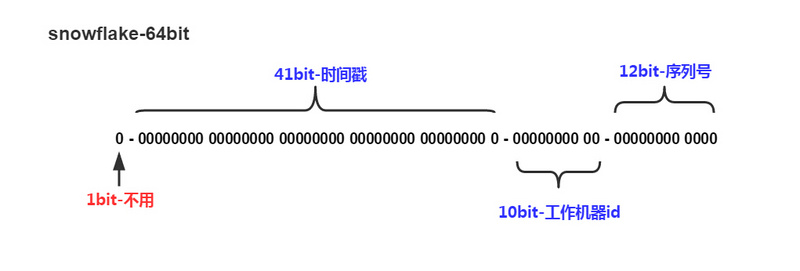
\includegraphics[scale = 0.7]{snowflake}\\
	\caption{SnowFlake 结构}
	\label{fig.snowflake}
\end{figure}

\begin{itemize}
\item 1位,不用.二进制中最高位为1的都是负数,但是我们生成的id一般都使用整数,所以这个最高位固定是0
\item 41位,用来记录时间戳(毫秒).
	\begin{itemize}
	\item $41$位可以表示$2^{41} − 1$个数字
	\item 如果只用来表示正整数(计算机中正数包含0),可以表示的数值范围是:$0$ 至 $2^{41} − 1$, 减1是因为可表示的数值范围是从0开始算的,而不是1. 转化成单位年则是$(2^{41} − 1) / (1000 \times 3600 \times 24 \times 365) = 69$年
	\end{itemize}
\item 10位,用来记录工作机器id.
	\begin{itemize}
	\item 可以部署在$2^{10} = 1024$个节点,包括5位datacenterId 和5位workerId
	\item 5位(bit)可以表示的最大正整数是$2^5 − 1 = 31$,即可以用$0,1,2,3,....31$这$32$个数字,来表示不同的datecenterId或workerId
	\end{itemize}
\item 12位,序列号,用来记录同毫秒内产生的不同id.
	\begin{itemize}
	\item 12位(bit)可以表示的最大正整数是$2^{12} − 1 = 4095$, 即可以用$0,1,2,3,....4094$这$4095$个数字,来表示同一机器同一时间截(毫秒)内产生的4095个ID序号
	\end{itemize}
\end{itemize}

SnowFlake可以保证:
\begin{itemize}
\item 所有生成的id按时间趋势递增
\item 整个分布式系统内不会产生重复id(因为有datacenterId和workerId来做区分)
\end{itemize}

\href{https://segmentfault.com/a/1190000011282426}{理解分布式id生成算法SnowFlake}

